\documentclass{llncs}

\usepackage{graphicx,array, rotating, ltablex}
\usepackage{multirow}
\usepackage[unicode]{hyperref}
\usepackage[colorinlistoftodos]{todonotes}

\graphicspath{{figures/}}
\newcolumntype{x}[1]{>{\centering\arraybackslash\hspace{0pt}}p{#1}}

\newcommand{\webdataset}{http://imageclef-lifelog.computing.dcu.ie/2017/}
\newcommand{\websitetask}{http://www.imageclef.org/2017/lifelog}

\newcommand{\oldtext}[1]{\textit{[To be rephrased: #1]}}

\hypersetup{
  colorlinks,
  breaklinks=true,
  citecolor=blue,
  linkcolor=blue,
  urlcolor=blue,
  %hyperfootnotes=false,
  pdfauthor={D.T. Dang-Nguyen et al.},
  pdftitle={Insights Discovery from Cloud-based Application Usage Data},
  pdfsubject={Report},
  pdfkeywords={ImageCLEF, CLEF labs, Lifelog}
}

\begin{document}

\title{Getting Insights from Cloud-based Applications: An Overview of Analytical Solutions}
\titlerunning{Insights Discovery from Cloud-based Application Usage Data}
\toctitle{Insights Discovery from Cloud-based Application Usage Data}

\authorrunning{D.T. Dang-Nguyen et al.}
\tocauthor{D.T. Dang-Nguyen et al.}

\author{Duc-Tien~Dang-Nguyen\inst{1} \and Markus Helfert\inst{1} }

\institute{LERO, Dublin City University\\ \email{\{duc-tien.dang-nguyen, markus.helfert\}@dcu.ie} 
}

\maketitle

\setcounter{footnote}{0}

\begin{abstract}
This reports summarises state-of-the-art approaches for usage analytics of cloud-based application from usage data and point out the potential applications of this novel research direction.
\end{abstract}

\section{Introduction}\label{sec:Introduction}
%
Analytical solutions refer to the use of various analysis
techniques (data mining, machine learning, reasoning, and etc.) to extract useful knowledge and insights from large data set. For example, enterprises can use analysis techniques to understand customers and predict which customers are least likely to quit, or most likely to respond to a particular offer based on their profiles, comments, and memberships they subscribe to. Moreover, the resulting predictions can be used to generate lists of target customers or cases of interest, as input for strategic planning, or can be integrated into the context
of other enterprise applications. Such analytical
solutions are considered as increasingly important tools for modern enterprise to get an informational advantage, and have evolved from a matter of choice to a necessity in some crowded and competitive business landscapes. 

In this report, we summarise the big picture of how analytical solutions can be applied in cloud-based environments and answer some basis questions: 
\begin{itemize}
	\item ``What are the usage data?"
	\item ``What kind of insights can we get from the extracted data?"
	\item ``What kind of analytical techniques should be applied?"
\end{itemize}

In order to answers these questions, let us recall the scenario of the cloud-based picture. Cloud providers deliver the same service to different customers, which share physical and/or virtual resources transparently. A cloud-based application lets customers (tenants) share the same hardware resources, by offering them one shared application and database instance, while allowing them to configure the application to fit their needs as if it runs on a dedicated environment []. End-users or consumers interact with the cloud applications through various interfaces (those being web browsers, mobile applications, and command-line interfaces). Cloud services allows different users to share computing and virtual resources transparently, meanwhile guaranteeing substantial cost savings []. The Infrastructure as a Service (IaaS) model offers computer - physical or virtual machines - and other resources, such as raw block storage, file or object storage, virtual local area networks (VLANs), IP addresses, and firewalls. In the Software as a Service (SaaS) model, users can access applications and data. The more resources are managed by cloud providers, the more resources are shared by multiple different users. Extraction of usage data of the features provided by the cloud applications could help developers and architects to make an informed decision for the development/improvement of functionalities of the system according to end-user usage patterns []. 

As summary, there are mainly three sources of usage data can be extracted: the system logs from the cloud services, the application logs, and the logs from the VMs. Fig.~\ref{fig:schema} shows a summary of the three main sources of usage data and the answers for the above questions. The next part of this report, some criteria for the data will be draw and 


\begin{figure}[t!]
	\centering
	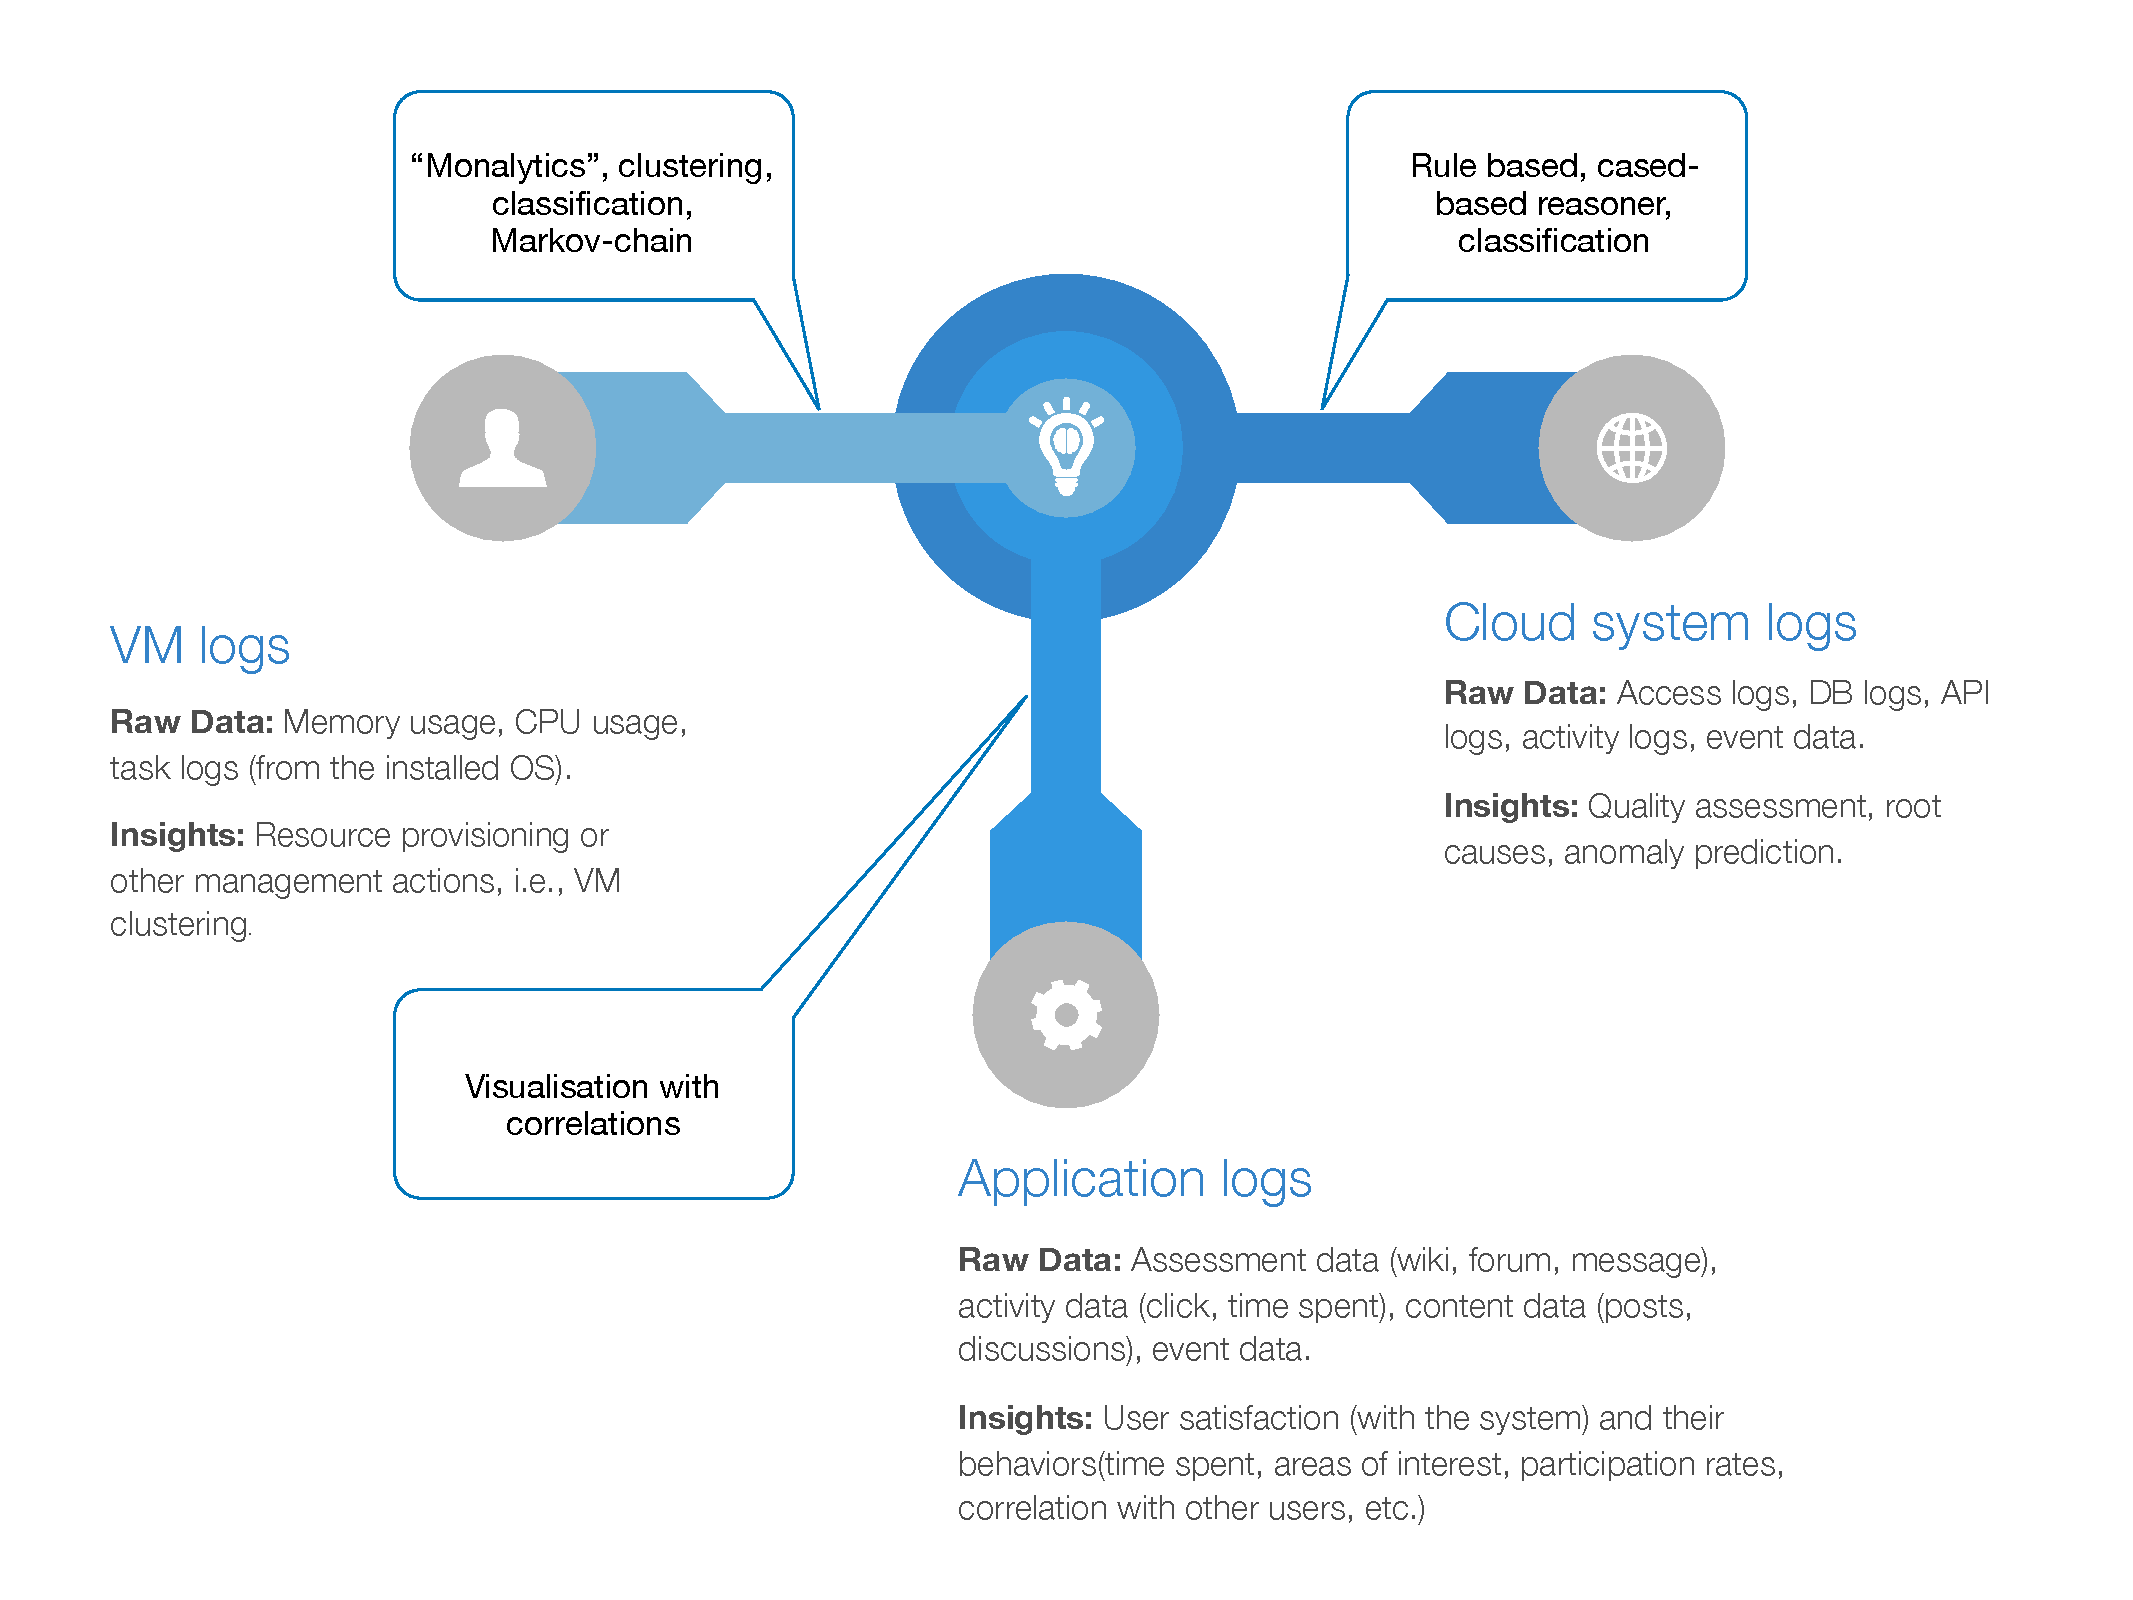
\includegraphics[width=\linewidth]{summary}
	\caption{Three main sources of usage data in cloud-based environment.}
	\label{fig:schema}
\end{figure}








%

\section{Basic Questions}

\section{Criteria}

Monitoring and Analytic methods have emerged as promising and inevitable solutions in this context, but require precise real time monitoring data. Towards this goal, we assess practical aspects for effectivemonitoring of SLA-aware services hosted inCloud. We present two real-world application scenarios for deriving requirements and present the prototype of ourMonitoring andAnalytics framework. We claimthat thiswork provides necessary foundations for researching SLA-aware root cause analysis algorithms under realistic setup.

Today more and more (monolithic) applications are decomposed into smaller components which are then executed as services on virtualized platforms con- nected via network communication and orchestrated to deliver the desired functionality. While the foun- dations for decomposing, executing and orchestrat- ing were well settled over the past decade, allocating the needed resources for and steering the execution of components to deliver the requiredQuality of Service (QoS) is an active area of research. A critical aspect of steering complex service-based applications on vir- tualized platforms is effective, non-intrusive, low- footprint monitoring of key performance indicators at different provisioning tiers typically Infrastructure- as-a-Service, Platform-as-a-Service and Software-as- a-Service. These key performance indicators are assessed to verify that a Service Level Agreement (SLA) between a customer and a provider ismet. Ide- ally, the assessment goes beyond simply detecting vi- olations of the agreed terms, but tries to predict and pre-empt potential violations. The provider enacts counter-measures to prevent or resolve the violation if
It it does occur. Deriving effective counter-measures re- quires precise monitoring information spanning mul- tiple tiers of the virtualized platform and analysis of monitoring data to identify the root cause(s) of per- formance problems.

Monitoring systems have been used for decades
in different computing paradigms. Monitoring solu- tions for previous computing paradigms pose signifi- cant limitations for their widespread adoption in large scale, virtual platforms. The major obstacles with these monitoring techniques are, their high perfor- mance overhead, reliability, isolation, limited scala- bility, reliance on proprietary protocols and technolo- gies.

Common performance diagnosis procedures de-
pend on system administrator’s domain knowledge and associated performance best practices. This pro- cedure is labor intensive, error prone, and not feasi- ble for virtual platforms. The prior art on detecting and diagnosing faults in computing systems can be re- viewed in (Appleby et al., 2001) (Molenkamp, 2002) (Agarwal et al., 2004) (Chen et al., 2002)(Barham et al., 2003). These methods do not consider virtual- ization technologies and are inappropriate for rapidly changing, large scale virtual platforms that by very nature require effective automated techniques forQoS fault diagnosis.

Our research motivations are to study the effec-
tiveness and practicality of different techniques for performance problem diagnosis and SLA based re- source management of virtual platforms. This is very well applicable to Cloud Computing where efficient monitoring is essential to accomplish these tasks. The remainder of this paper is organized as follows. Sec- tion 2 presents scenarios of our interest againstwhich in Section 3, we derive requirements for monitoring and analytics. Based on this, in Section 4, we present our Monitoring and Analytics framework prototype developed as part of the GWDG Cloud Infrastructure. Section 5 describes related work and finally, we con- clude the paper in Section 6 with a summary and fu- ture plan.



\section{The Proposed Usage Analytics Methods}

\subsection{Usage Analytics from VM Logs}
Learning Management Systems (LMS) or Virtual Learning Environments (VLE) are widely used and have become part of the common toolkits of educators (Schroeder, 2009). One of the main goals of the integration of traditional teaching methods with technology enhancements is the improvement of teaching and learning quality in large university courses with many students. But does utilizing a VLE automatically improve teaching and learning? In our experience, many teachers just upload existing files, like lecture slides, handouts and exercises, when starting to use a VLE. Thereby availability of learning resources is improved. For improving teaching and learning it could be helpful to create more motivating, challenging, and engaging learning materials and e.g., collaborative scenarios to improve learning among large groups of students. Teachers could e.g., use audio and video recordings of their lectures or provide interactive, demonstrative multimedia examples and quizzes. If they put effort in the design of such online learning activities, they need tools that help them observe the consequences of their actions and evaluate their teaching interventions. They need to have appropriate access to data to assess changing behaviors and performances of their students to estimate the level of improvement that has been achieved in the learning environment.
With the establishment of TEL, a new research field, called Learning Analytics, is emerging (Elias, 2011). This research field borrows and synthesizes techniques from different related fields, such as Educational Data Mining (EDM), Academic Analytics, Social Network Analysis or Business Intelligence (BI), to harness them for converting educational data into useful information and thereon to motivate actions, like self-reflecting ones previous teaching or learning activities, to foster improved teaching and learning. The main goal of BI is to turn enterprise data into useful information for management decision support. However, Learning Analytics, Academic Analytics, as well as EDM more specifically focus on tools and methods for exploring data coming from educational contexts. While Academic Analytics take a university-wide perspective, including also e.g., organizational and financial
issues
(Campbell \& Oblinger, 2007), Learning Analytics as well as EDM focus specifically on data about teaching and learning.
Siemens (2010) defines Learning Analytics as “the use of intelligent data, learner-produced data, and analysis models to discover information and social connections, and to predict and advise on learning.” It can support teachers and students to take action based on the evaluation of educational data. However, the technology to deliver this potential is still very young and research on understanding the pedagogical usefulness of Learning Analytics is still in its infancy (Johnson et al., 2011b; Johnson et al., 2012).
ISSN

\subsection{Usage Analytics from Application Logs}
With the increasing scale and complexity of software
systems, it has become more and more difficult for system operators to understand the behaviors of software systems for tasks such as system problem diagnosis. For example, system operators need to understand system behaviors to figure out why a software system is in the current status. With such an understanding, they can choose the right operations to achieve the desired goal. System behaviors include a series of actions executed by the system and the corresponding changes in the system states. Although operators usually investigate a system starting from a specific state of interest, e.g., a hang state or failure state, contextual information for reaching that state is critical for identifying why the system runs in that state. Such contextual information includes how previous actions are executed by the system, what the historical system states are before running into the state of interest, what the input data is, etc.

To help system operators understand a system’s behaviors,
three main sources of information are available: system documentations, source code, and program logs. Ideally, system documentations are expected to provide detailed and up-to-date information about the system. However, in practice, system documentations are often incomplete, outdated, or even unavailable. Many systems are not well documented due to tight release schedules or poor project management. Program source code is another source that provides accurate and detailed information about a system. However, the source code of the system is not always available to system operators. For example, in many cases, a system may include third-party components whose source code is not available. The information provided by program logs [1] has been the
most widely used source for system operators to understand system behaviors, especially for a large-scale online system. Program logs contain a wealth of information to help manage systems. Most systems print out program logs during their executions to record system runtime actions and states that can directly reflect system runtime behaviors. System operators usually use these logs to track a system to detect and diagnose system anomalies.

However, there are challenges in analyzing program logs in
order to understand a system’s behaviors. The program logic of a system usually has a lot of branches, and thus the system’s behaviors may be quite different under different input data or environmental conditions. Knowing the execution behavior under different inputs or configurations can greatly help system operators to understand system behaviors. However, there may be a large number of different combinations of inputs or parameters under different system behaviors. Such complexity poses difficulties for analyzing contextual information related to the state of interest. To address this challenge, in this paper, we propose a new
approach for the contextual analysis of program logs to better understand a system’s behaviors. In particular, we use execution patterns to represent the execution structures reflected by program logs, and propose an algorithm to mine execution patterns from the program logs. The mined execution patterns correspond to different execution paths of the system. Based on the execution patterns, our approach further learns the essential contextual factors (e.g., occurrences of specific program logs with specific parameter values) that cause a specific branch or path to be executed by the system. The mining and learning results can help system operators understand the execution logic and behaviors of a software system for their various maintenance tasks such as system problem diagnosis. This paper makes the following research contributions: ? We conduct Formal Concept Analysis (FCA) [4] to analyze log messages, and construct a concept lattice graph. The learned graph is used to mine execution patterns and to model relationships among different execution patterns. Such relationships represent branch structures in the program execution logic.
? Based on the lattice graph, we propose a feature extraction technique and use decision trees to learn branch conditions. The learned branch conditions reveal essential contextual factors that determine which code branches the system will take at bifurcation points.

Ahuge wealth of various data exists in the software development
process, and hidden in the data is information about the quality of software and services as well as the dynamics of software develop- ment. With various analytic technologies (e.g., data mining, ma- chine learning, and information visualization), software analytics is to enable software practitioners1 to perform data exploration and
1Software

analysis in order to obtain insightful and actionable information for data-driven tasks around software and services2. Insightful information is information that conveys meaningful
and useful understanding or knowledge towards performing the tar- get task. Typically insightful information is not easily attainable by directly investigating the raw data without aid of analytic technolo- gies. Actionable information is information upon which software practitioners can come up with concrete solutions (better than ex- isting solutions if any) towards completing the target task. Developing a software analytic project typically goes through it-
erations of the life cycle of four phases: task definition, data prepa- ration, analytic-technology development, and deployment and feed- back gathering. Task definition is to define the target task to be as- sisted by software analytics. Data preparation is to collect data to be analyzed. Analytic-technology development is to develop prob- lem formulation, algorithms, and systems to explore, understand, and get insights from the data. Deployment and feedback gather- ing involves two typical scenarios. One is that, as researchers, we have obtained some insightful information from the data and we would like to ask domain experts to review and verify. The other is that we ask domain experts to use the analytic tools that we have developed to obtain insights by themselves. Most of the times it is the second scenario that we want to enable. Among various analytic technologies,machine learning is awell-
recognized technology for learning hidden patterns or predictive models from data. It plays an important role in software analyt- ics. In this position paper, we argue that when applying analytic technologies in practice of software analytics, one should

incorporate a broad spectrum of domain knowledge and ex- pertise, e.g.,management, machine learning, large-scale data processing and computing, and information visualization;
• investigate how practitioners take actions on the produced insightful and actionable information, and provide effective support for such information-based action taking.
Our position is based on a number of software analytic projects
that have been conducted at the Software Analytics (SA) group3 at Microsoft Research Asia (MSRA) in recent years (in the rest of this paper, we refer to members of the software analytic projects at MSRA as the SA project teams). These software analytic projects have undergone successful technology transferwithinMicrosoft for enabling informed decision making and improving quality of soft- ware and services. We expect that our position will provide useful
2We


\subsection{Usage Analytics from Cloud-based Systems}
	
\section{Challenge}

There are two main categories of challenges to overcome in or-
der to achieve the stated objectives. The first category is rooted from the characteristics of the data being analyzed with analytic technologies. Data scale. Typical data in software analytics is of large scale,
e.g., due to the large scale of software being developed and the large size of software development teams. Some tasks require to analyze division-wide or even company-wide code bases, which are far be- yond the scope of a single code base (e.g., when conducting code- clone detection [2]). Some tasks require to analyze a large quantity of (likely noisy) data samples within or beyond a single code base (e.g., when conducting runtime-trace analysis [3]). Although lack- ing data samples may not be an issue in this context of machine learning, the large scale of data poses challenges for data process- ing and analysis, including learning-algorithm design and system building. Data complexity. Typical data in software analytics is of high
complexity, which is partly due to the high complexity of software being developed. For example, runtime traces fromdistributed sys- tems [3] need to be correlated, while traces frommultiple threads [7] need to be split. System logs [3] include unstructured textual in- formation. There could be high dependencies across traces and noises among traces. In addition, real-world usage data produced from in-field operations offers substantial opportunities for various tasks such as debugging (e.g., those assisted by the Microsoft Er- ror Reporting system [4]). In addition to high complexity, such data is typically distributed and often partial (e.g., collected with sampling-based techniques to reduce runtime overhead). All these characteristics pose challenges for analytic technologies such as machine learning. The second category is rooted from the characteristics of the
tasks being assisted by software analytics. Focus on ultimate tasks being assisted. Among tasks assisted
by software analytics, some tasks are intermediate tasks and some are ultimate tasks. Usually intermediate tasks produce information toward solving ultimate tasks. For example, code-clone detection is considered as an intermediate task, which produces information towards refactoring and defect detection that are ultimate tasks.

Such focus on ultimate tasks requires the mandatory inclusion of the phase of deployment and feedback gathering in the life cycle of a software analytic project. Unlike most previous research on code-clone detection, we should not stop at measuring the preci- sion and recall of detected clones; rather, we should push further to accomplish that the detected clones could effectively help address ultimate tasks such as refactoring and defect detection, and should measure such benefits in evaluations. Engagement of customers during the development process of a
software analytic project. It is well recognized that engaging cus- tomers is a challenging task especially in the context of software engineering tools. Customers may have resistance to proposed changes (due to analytic-tool adoption) on their existing way of carrying out a task. In addition, due to tight development sched- ule, they may not be able to invest time on gaining understanding of the best/worst scenarios for applying an analytic tool. However, developing a software analytic project typically needs the engage- ment of customers in iterations of the four phases in the project life cycle, e.g., to get better understanding on the tasks and domain knowledge. Among the phases, especially the phase of deployment and feedback gathering, it is crucial for the produced analytic tools to have good usability, e.g., providing effective visualization and manipulation of analysis results.

Unfortunately, despite the advantages provided by analytical solutions, the solution implementation is usually very costly, which hinders enterprises, especially the SMBs (Small and Medium Business), to start such projects. Typically, an enterprise is required to first build a large
storage system to store huge volumes of data collected from various data sources and channels; after that, the enterprise should buy expensive analytics software, and a large number of server machines, because the analytical programs often need mining huge amounts of data or executing complex learning algorithms. Moreover, the computational resource demand pattern of analytical solutions may be uneven with spikes (e.g., predicting product sale when a financial quarter is over or some unusual events happen), which means the enterprise has to pay a lot to maintain the complex software and hardware only for occasional usages. As a result, the systematical adoption of analytical
solution is currently
limited to only a small number of large enterprises. On the other hand, the analytical solution vendors also
find it is difficult to deliver cost-effective solutions. Because analytical solutions
require continuous model validation,
tuning, and update according to the changing business context,
it is hard for the solution vendors to control
the
travel expenditure in sending analysts to conduct incremental services in the customer site. In a word, a cost-effective delivery model becomes an
important
issue to accelerate the prevalence of analytical
solutions. Currently, SaaS delivery model is well-studied to enable business clients consume applications at a low cost based on their usage [1], and cloud computing is considered as a promising technology to provide on demand storage and computational resources flexibly [2]. Accordingly, there are several
relevant research efforts which have focused on
leveraging these technologies to facilitate analytical solution delivery [3][4]. However, most of the projects are ad-hoc, that is, each of them is
specific to a certain analytical
application domain, and there is still lack of a comprehensive study to identify the differences between existing analytical solution delivery and analytics-as-a-service delivery, as well as a technical framework to handle the technical challenges introduced by the new delivery model.


\section{Realising the Potential}
	
\section{Conclusions}



\bibliographystyle{splncs03}
\bibliography{ref}
%
%\newpage
\appendix

\section{Topics List 2017}\label{app:topics}
%
The following tables present the descriptions of 51 search topics for the ImageCLEF 2017 LifeLog Retrieval and Summarization Tasks.
\input{tables/devset_lrt_topics_descr}
\input{tables/testset_lrt_topics_descr}
\input{tables/devset_lst_topics_descr}
\input{tables/testset_lst_topics_descr}
%
\end{document}